\chapter{Περιγραφή του προβλήματος}\label{ch:problem}

\section{Ο διαγωνισμός της Wyze: κίνητρα και δεδομένα}\label{sec:wyze-comp}
Στο πλαίσιο της ανάπτυξης καινοτόμων τεχνολογιών στον χώρο του Διαδικτύου των Πραγμάτων, η τεχνολογική εταιρεία Wyze διεξήγαγε έναν διαγωνισμό με σκοπό τη δημιουργία αλγορίθμων έξυπνης σύστασης κανόνων για IoT συσκευές. Στόχος αυτών των αλγορίθμων είναι να προτείνουν στους χρήστες που κατέχουν τέτοιες συσκευές (π.χ. κάμερες, έξυπνες λάμπες, αισθητήρες κίνησης κ.ά.) νέους, προσωποποιημένους τρόπους να αυτοματοποιήσουν τη λειτουργία τους, βασιζόμενοι στα μοτίβα και το ιστορικό χρήσης τους. Έχοντας πολυετή παρουσία στον χώρο του IoT, η Wyze διαμόρφωσε ένα σύνολο δεδομένων που προέρχεται από περισσότερους από 300.000 πραγματικούς χρήστες και περιλαμβάνει πάνω από 1.000.000 κανόνες \cite{noauthor_wyzelabsrulerecommendation_nodate}. Ωστόσο ένας αλγόριθμος που επεξεργάζεται αυτά τα δεδομένα και εξάγει μοτίβα χρήσης προκαλεί έντονη ανησυχία για την ιδιωτικότητα και την προστασία των προσωπικών δεδομένων των χρηστών. Για τον λόγο αυτό, προτάθηκε μία εναλλακτική προσέγγιση στο πρόβλημα μέσω της Ομοσπονδιακής Μάθησης \cite{yao_fedrule_2022}. Η μέθοδος αυτή εξασφαλίζει ότι το τοπικό μοντέλο εκπαιδεύεται αποκλειστικά στη συσκευή του εκάστοτε χρήστη, ανταλλάσσοντας με τον κεντρικό server μόνο τις αναβαθμισμένες παραμέτρους και ποτέ τα ίδια τα ευαίσθητα δεδομένα.

Η Wyze μοντελοποίησε τους κανόνες του κάθε χρήστη μέσω μιας τριπλέτας της μορφής «συσκευή – κανόνας – συσκευή». Σύμφωνα με αυτή τη δομή, όταν η πρώτη συσκευή βρεθεί σε μία συγκεκριμένη κατάσταση (π.χ. ένας αισθητήρας εντοπίζει κίνηση), τότε πυροδοτείται η δράση της δεύτερης συσκευής (π.χ. ένας λαμπτήρας ανάβει). Το παραπάνω παράδειγμα, δηλαδή, εκφράζεται ως η τριπλέτα «αισθητήρας κίνησης – εντοπισμός κίνησης → ενεργοποίηση – λαμπτήρας».

\begin{figure}[htbp]
  \centering
  
\includegraphics[width=0.8\linewidth]{./assets/images/triplet}
  \caption[Η τριπλέτα συσκευή--κανόνας--συσκευή]{Η τριπλέτα «συσκευή -- κανόνας -- συσκευή»: μια συσκευή-πηγή (κάμερα Α) σε συγκεκριμένη κατάσταση (ανίχνευση κίνησης) πυροδοτεί μια δράση (άναψε) σε μια συσκευή-στόχο (λαμπτήρας Β).}
  \label{fig:triplet}
\end{figure}

Επειδή το σύνολο δεδομένων της Wyze προέρχεται από πραγματικούς χρήστες, αντικατοπτρίζει αναπόφευκτα την τεράστια ποικιλομορφία στον τρόπο με τον οποίο διαφορετικοί άνθρωποι χρησιμοποιούν το IoT οικοσύστημά τους. Αυτό έχει ως αποτέλεσμα τα δεδομένα να μην ακολουθούν Ανεξάρτητες και Ταυτόσημα Κατανεμημένες (IID) κατανομές, να είναι δηλαδή ετερογενή, όπως αναλύθηκε στην \autoref{ssec:fl}. Συγκεκριμένα, παρατηρήθηκε ότι το μεγαλύτερο μέρος των χρηστών κατέχει πολύ λίγες συσκευές και έχει δημιουργήσει ελάχιστους κανόνες μεταξύ τους, δημιουργώντας μία κατανομή μακράς ουράς (long-tailed distribution), όπως καταδεικνύεται στο \autoref{fig:dataset-stats}. Η κατάσταση αυτή εισάγει έντονη αραιότητα στα δεδομένα. Η εξαγωγή χρήσιμων μοτίβων από ένα τόσο αραιό και ετερογενές σύνολο καθιστά την εκπαίδευση ενός μοντέλου μηχανικής μάθησης σαφώς δυσκολότερη απ' ό,τι σε πυκνά σύνολα δεδομένων, πόσο μάλλον όταν αυτή η εκπαίδευση πρέπει να πραγματοποιηθεί ομοσπονδιακά.

\section{Μοντελοποίηση του προβλήματος}\label{sec:problem-model}
Όπως εξετάστηκε και στην \autoref{sec:recsys}, το πρόβλημα της Wyze εντάσσεται στην ευρύτερη κατηγορία των συστημάτων σύστασης. Σκοπός των συστημάτων αυτών είναι η πρόβλεψη μιας νέας πληροφορίας (π.χ. η επόμενη ταινία που θα ενδιέφερε έναν χρήστη), βασιζόμενη τόσο στα υπάρχοντα δεδομένα του ίδιου του χρήστη (ιστορικό θεάσεων), όσο και σε δεδομένα χρηστών με παρόμοια συμπεριφορά.

Η κυρίαρχη μέθοδος μοντελοποίησης τέτοιων προβλημάτων, η οποία διαδόθηκε ευρέως μέσω του διαγωνισμού της εταιρείας Netflix το 2009, βασίζεται στην παραγοντοποίηση πινάκων (matrix factorization) \cite{koren_matrix_2009}. Σε αυτή την προσέγγιση, οι χρήστες και τα αντικείμενα (π.χ. ταινίες) αναπαριστώνται μέσω ενός πίνακα, όπου κάθε γραμμή αντιστοιχεί σε έναν χρήστη και κάθε στήλη σε ένα αντικείμενο. Ο πίνακας αυτός είναι μερικώς συμπληρωμένος (π.χ. στον χρήστη 3 άρεσαν οι ταινίες 2, 5 και 7, δεν άρεσε η ταινία 1 και δεν έχει αξιολογήσει τις υπόλοιπες). Στόχος είναι η πρόβλεψη των κενών τιμών του πίνακα, αξιοποιώντας τα λανθάνοντα μοτίβα που εμφανίζονται στο σύνολό του. Οι τεχνικές που χρησιμοποιούνται για αυτή τη συμπλήρωση ποικίλλουν, ωστόσο η ανάλυσή τους εκφεύγει του σκοπού της παρούσας εργασίας.

Υπάρχουν μερικές σημαντικές λεπτομέρειες του μοντέλου αυτού οι οποίες το καθιστούν μη λειτουργικό για το περιβάλλον των IoT συσκευών της Wyze \cite{yao_fedrule_2022}. Αρχικά, οι σχέσεις μεταξύ των έξυπνων συσκευών είναι υπερβολικά περίπλοκες για να αποτυπωθούν αποτελεσματικά σε έναν απλό πίνακα (user-item matrix). Για παράδειγμα, ενώ ένα σύστημα πρόβλεψης αγορών μοντελοποιεί κυρίως απλές δυαδικές σχέσεις (π.χ. αγορά/μη αγορά), μία IoT αλληλεπίδραση ενέχει προϋποθέσεις και λογική (π.χ. «αν η κάμερα εντοπίσει κίνηση, τότε ο λαμπτήρας ανάβει» ή «αν η ώρα είναι 17:00, τότε το ρολό σκίασης κατεβαίνει»). Επιπλέον, ένας χρήστης συχνά κατέχει πολλαπλές συσκευές του ίδιου ακριβώς τύπου (π.χ. τρεις έξυπνους λαμπτήρες σε διαφορετικά δωμάτια). Για να διαχωριστούν αυτές σε έναν πίνακα, θα απαιτούνταν ξεχωριστές στήλες για την καθεμία, γεγονός που θα καθιστούσε τον συνολικό πίνακα για εκατοντάδες χιλιάδες χρήστες όχι μόνο υπολογιστικά τεράστιο, αλλά και εξαιρετικά αραιό. Τέλος, η διατήρηση ενός κεντρικού πίνακα που συγκεντρώνει όλη την πληροφορία για τις συσκευές όλων των χρηστών εγείρει σοβαρούς κινδύνους ιδιωτικότητας, καθώς μία ενδεχόμενη παραβίαση αρκεί για να εκθέσει ευαίσθητα προσωπικά δεδομένα, όπως συνέβη στο παρελθόν σε αντίστοιχες πλατφόρμες, συμπεριλαμβανομένης της Wyze \cite{geekwire_wyze_2019}.

Για τον λόγο αυτό προτάθηκε η εναλλακτική αναπαράσταση των χρηστών και των συσκευών τους μέσω γράφων. Όπως παρουσιάστηκε συνοπτικά στην \autoref{sec:graphs}, κάθε χρήστης $u_k \in \mathcal{U}$ εκφράζεται από έναν γράφο $\mathcal{G}_k = \{\mathcal{V}_k, \mathcal{X}_k, \mathcal{E}_k\}$. Σε αυτόν, οι κόμβοι $\mathcal{V}_k$ αναπαριστούν τις διαφορετικές συσκευές του χρήστη, οι ακμές $\mathcal{E}_k$ αναπαριστούν τους ενεργούς κανόνες μεταξύ τους (τη δομή «συσκευή – κανόνας – συσκευή»), και τα χαρακτηριστικά $\mathcal{X}_k$ περιγράφουν τις ιδιότητες κάθε κόμβου (λειτουργίες, δυνατές συνδέσεις, πιθανές καταστάσεις). Η προσέγγιση αυτή επιλύει εγγενώς τις αδυναμίες του πίνακα: η πολυπλοκότητα των κανόνων μεταξύ συσκευών εκφράζεται ελεύθερα μέσω των ακμών που τις συνδέουν, κάθε χρήστης μπορεί να έχει όσες συσκευές του ίδιου τύπου θέλει χωρίς να επηρεάζει τους άλλους χρήστες, και κυρίως, ο κάθε χρήστης διατηρεί τον δικό του απομονωμένο γράφο, προστατεύοντας έτσι την τοπολογία του έξυπνου σπιτιού του.

\begin{figure}[htbp]
  \centering
  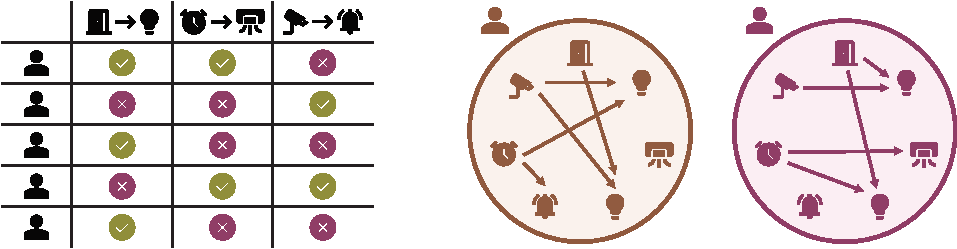
\includegraphics[width=\linewidth]{./assets/images/matrix-vs-graph}
  \caption[User-item matrix vs. γράφος]{Οι δύο αναπαραστάσεις του προβλήματος: ο user-item πίνακας του matrix factorization (αριστερά) έναντι της αναπαράστασης ανά χρήστη με γράφο (δεξιά).}
  \label{fig:matrix-vs-graph}
\end{figure}

Βάσει αυτού του ανανεωμένου μοντέλου, ο στόχος ορίζεται με σαφήνεια: η πρόταση νέων κανόνων (ακμών) μεταξύ των υπαρχουσών συσκευών (κόμβων) του κάθε χρήστη, αξιοποιώντας την αφηρημένη γνώση που εξάγεται τόσο από τον δικό του γράφο όσο και από το δίκτυο των υπολοίπων. Αυτό υλοποιείται μαθηματικά μέσω μιας διπλής διαδικασίας: πρώτον, του node embedding (βλ. \autoref{sec:gnn}), δηλαδή της κωδικοποίησης των χαρακτηριστικών $\mathcal{X}_k$ και της τοπολογίας σε διανυσματικές αναπαραστάσεις που περιγράφουν τις ιδιότητες κάθε συσκευής, και δεύτερον, της πρόβλεψης συνδέσεων (link prediction), η οποία αξιολογεί τα παραγόμενα διανύσματα για να προτείνει τις νέες ακμές με τη μεγαλύτερη πιθανότητα να φανούν χρήσιμες στον τελικό χρήστη.

\section{Διαχείριση δεδομένων}\label{sec:data}
Το μοντέλο της Wyze παρουσιάζει δύο θεμελιώδεις προκλήσεις, εγγενείς στην φύση των πραγματικών IoT δεδομένων των χρηστών. Η πρώτη αφορά την ακραία αραιότητα των δεδομένων. Ένας μέσος χρήστης κατέχει έναν αριθμό συσκευών (π.χ. 8 έξυπνους λαμπτήρες και μία κάμερα), αλλά έχει διαμορφώσει ελάχιστους ενεργούς κανόνες (ακμές) μεταξύ τους (π.χ. 2 κανόνες για τον χειρισμό του φωτισμού και άλλον έναν για την παρακολούθηση της κάμερας). Συγκριτικά, σε έναν πλήρως συνδεδεμένο, κατευθυνόμενο γράφο $n=8$ κόμβων, οι πιθανές ακμές είναι $n(n-1)=56$. Σε ένα σύστημα πρόβλεψης συνδέσεων, το μοντέλο καλείται να ταξινομήσει κάθε πιθανή ακμή, με την πλειονότητα του γράφου να ανήκει στην κλάση «μη σύνδεση» (στο παράδειγμά μας 53 από τις 56 δυνατές ακμές δεν έχουν κάποιον κανόνα). Εάν από τις 56 πιθανές ακμές μόνο οι 3 είναι υπαρκτές, προκύπτει εντονότατη ανισορροπία κλάσεων (class imbalance) \cite{he_learning_2009}. Συνέπεια αυτού είναι το «παράδοξο της ακρίβειας» (accuracy paradox): το μοντέλο τείνει να προβλέπει σταθερά την κλάση της «μη σύνδεσης», επιτυγχάνοντας φαινομενικά εξαιρετική ακρίβεια $53/56 \approx 94.6\%$, χωρίς όμως να εξάγει καμία ουσιαστική γνώση για το σύστημα σύστασης.

Για την αντιμετώπιση αυτής της πρόκλησης, το σύστημα FedRule της Wyze εισάγει τη μέθοδο της δειγματοληψίας αρνητικών ακμών (negative sampling) \cite{he_learning_2009}. Κατά την τοπική εκπαίδευση, το μοντέλο δεν εξετάζει το σύνολο των συνδέσεων του γράφου, αλλά ένα τεχνητά περιορισμένο υποσύνολό τους, το οποίο περιλαμβάνει όλες τις θετικές ακμές (τους πραγματικούς κανόνες, στο παράδειγμά μας, τρεις) μαζί με ένα τυχαίο υποσύνολο αρνητικών ακμών, σε κάποια θεμιτή αναλογία (π.χ. 1:1, έστω στο παράδειγμά μας, τέσσερις ακμές). Μέσω αυτής της τεχνητής εξισορρόπησης του δείγματος, η κλάση της «μη σύνδεσης» παύει να είναι συντριπτικά κυρίαρχη. Το μοντέλο δεν μπορεί πλέον να προτείνει αφελώς τον κανόνα «μη σύνδεση», διότι η ακρίβεια αυτής της πρόβλεψης είναι πολύ κακή (εδώ $4/7 \approx 57.1\%$), και έτσι αναγκάζεται να εντοπίσει πραγματικά λανθάνοντα μοτίβα για να διαχωρίσει τις έγκυρες από τις άκυρες συνδέσεις, οδηγώντας σε χρήσιμες και ακριβείς συστάσεις.

Το δεύτερο πρόβλημα αφορά τη φύση των ετερογενών δεδομένων. Όπως αναφέρθηκε στην \autoref{sec:wyze-comp}, οι κατανομές δεδομένων μεταξύ των χρηστών δεν είναι ανεξάρτητες και ταυτόσημα κατανεμημένες (non-IID). Για παράδειγμα, ένας χρήστης μπορεί να διαθέτει αποκλειστικά έξυπνους λαμπτήρες, ενώ ένας άλλος κυρίως κάμερες ασφαλείας. Σε ένα καθεστώς ομοσπονδιακής μάθησης, όπου κάθε χρήστης εκπαιδεύει το δικό του τοπικό μοντέλο και πραγματοποιεί gradient descent με βάση τα δεδομένα που έχει στην διάθεσή του (βλ. \autoref{sec:fl}), αυτές οι αποκλίσεις στον όγκο και το είδος των δεδομένων αυξάνουν τη διακύμανση των κλίσεων των χρηστών, οδηγώντας το σύστημα σε client drift \cite{karimireddy_scaffold_2020} (βλ. \autoref{ssec:fl}).

Για να αντισταθμίσει την πρόκληση αυτή, η Wyze ενσωμάτωσε στον αλγόριθμό της μια τεχνική μείωσης της διακύμανσης (variance reduction), βασισμένη στην χρήση διορθωτικών παραμέτρων ελέγχου (control parameters) κατ' αντιστοιχία με τον αλγόριθμο FedGATE \cite{haddadpour_federated_2021}, στο πνεύμα και άλλων μεθόδων μείωσης διακύμανσης με παραμέτρους ελέγχου όπως το SCAFFOLD \cite{karimireddy_scaffold_2020}. Συγκεκριμένα, κάθε client $k$ διατηρεί τοπικά δύο παραμέτρους ελέγχου: την $\delta_{\theta_k}$ για το μοντέλο του GNN και την $\delta_{\phi_k}$ για το μοντέλο πρόβλεψης του κανόνα. Ανατρέχοντας πίσω στην ροή εκπαίδευσης της Ενότητας \ref{sec:fl}, παρατηρούμε την εξής αλλαγή: Κατά τον υπολογισμό των κλίσεων $g_{\theta_k}$ και $g_{\phi_k}$, το τοπικό μοντέλο δεν προχωρά σε άμεση ενημέρωση των βαρών του. Αντιθέτως, αφαιρεί από τις κλίσεις τις παραμέτρους $\delta_{\theta_k}$, $\delta_{\phi_k}$, παράγοντας έτσι διορθωμένες κλίσεις που αποτρέπουν την υπερβολική απόκλιση από το κεντρικό μοντέλο. Μετά το πέρας της τοπικής εκπαίδευσης, οι clients αποστέλλουν στον κεντρικό server μόνο τις συνολικές διαφορές των βαρών τους $\Delta_{\theta}$, $\Delta_{\phi}$. Ο server υπολογίζει τον μέσο όρο αυτών των διαφορών και τον μεταδίδει πίσω στους clients. Χρησιμοποιώντας αυτόν τον παγκόσμιο μέσο όρο, κάθε client αναπροσαρμόζει τις δικές του τοπικές παραμέτρους ελέγχου $\delta_{\theta_k}$ και $\delta_{\phi_k}$. Αυτή η διαδικασία συνεχούς διόρθωσης εξασφαλίζει ότι τα ετερογενή τοπικά μοντέλα διατηρούν κοινό προσανατολισμό, επιτρέποντας στο global μοντέλο να συγκλίνει γρήγορα και με σταθερότητα σε μία λύση αρκετά ικανοποιητική για όλους τους χρήστες.

\section{Το αρχικό μοντέλο της Wyze}\label{sec:wyze-baseline}
Μαζί με την δημοσίευση του paper της \cite{yao_fedrule_2022}, η Wyze διέθεσε ανοιχτά μία αρχική υλοποίηση \cite{yao_yh-yaofedrule_2025} για να χρησιμοποιηθεί ως βάση στον διαγωνισμό. Στόχος δεν ήταν η αυτούσια πειραματική απόδειξη των αποτελεσμάτων του paper, αλλά η παροχή ενός καθοδηγητικού πλαισίου προς τους διαγωνιζόμενους. Για αυτό τον λόγο παρατηρείται μία πολύ απλοποιημένη αρχιτεκτονική σε σχέση με αυτή που προτάθηκε στο paper.

\subsection{Το pipeline του μοντέλου}\label{ssec:pipeline}
\subsubsection{Προετοιμασία δεδομένων}
Τα σύνολα δεδομένων που δόθηκαν στους διαγωνιζόμενους απαρτίζονται από 16 διαφορετικές κατηγορίες συσκευών. Η υλοποίηση της Wyze αντιστοιχίζει ένα ID σε καθεμιά από αυτές τις κατηγορίες, αγνοώντας την κατηγορία “Cloud”, η οποία υπάρχει μόνο στο dataset των κανόνων και όχι σε αυτό των συσκευών. Στην συνέχεια, φιλτράρει όλες τις τριπλέτες «συσκευή – κανόνας – συσκευή» που εμφανίζονται λιγότερο από 10 φορές συνολικά, για να εκπαιδεύσει το μοντέλο σε δεδομένα που εμφανίζονται συχνά και όχι σε εξαιρέσεις, και δομεί το λεξιλόγιο των συσκευών και κανόνων για όλους τους χρήστες. Για την δημιουργία των γράφων κάθε χρήστη χρησιμοποιείται η βιβλιοθήκη Deep Graph Library (DGL) \cite{wang_deep_2019, dgl_software}. Κάθε συσκευή αναπαρίσταται από έναν κόμβο, με τον τύπο της (π.χ. κάμερα, πρίζα) να κωδικοποιείται ως ένα one-hot διάνυσμα features. Οι κανόνες αναπαρίστανται ως ακμές, με τους τύπους τους (etypes) να αντιστοιχούν στην εκάστοτε τριπλέτα «συσκευή – κανόνας – συσκευή». Αν ο γράφος κάποιου χρήστη καταλήξει με 2 ή λιγότερους κόμβους, τότε απορρίπτεται. Στην συνέχεια, οι κόμβοι κάθε χρήστη χωρίζονται σε ποσοστό 80\% για εκπαίδευση (training) και 20\% για αξιολόγηση (testing). Τέλος, πριν την διαδικασία του training, εφαρμόζεται negative sampling στους γράφους: ο αλγόριθμος αναλύει τον πίνακα γειτνίασης (adjacency matrix) κάθε γράφου, εντοπίζει ζεύγη κόμβων που δεν συνδέονται και επιλέγει τυχαία ένα υποσύνολο αυτών, ώστε να χρησιμεύσουν ως αρνητικά παραδείγματα (λανθασμένες συνδέσεις) κατά την εκμάθηση.

\subsubsection{Μοντέλα μηχανικής μάθησης}
Όπως περιγράφεται και στο paper, η αρχιτεκτονική αποτελείται από δύο διακριτά μέρη: ένα Graph Neural Network (GNN) για την κωδικοποίηση της πληροφορίας των γράφων μέσω embeddings, και ένα μοντέλο link prediction για την πρόταση νέων ακμών. Για το πρώτο μέρος, η υλοποίηση πειραματίζεται με τα μοντέλα GCN \cite{kipf_semi-supervised_2017}, GAT \cite{velickovic_graph_2018} και GraphSAGE \cite{hamilton_inductive_2017}. Όπως καταδεικνύεται στο ablation study (Ενότητα 4.5 του paper) \cite{yao_fedrule_2022}, το GraphSAGE υπερισχύει, κυρίως λόγω της στιβαρής διαχείρισης κόμβων με μηδενικό βαθμό εισόδου (0-in-degree nodes). Έτσι χρησιμοποιείται η δομή του GraphSAGE που αναφέρεται στο paper: 2 επίπεδα SAGEConv με mean aggregation και ReLU ενεργοποίηση μετά το πρώτο επίπεδο. Το δεύτερο στάδιο της υλοποίησης αξιοποιεί ένα κλασικό πλήρως συνδεδεμένο Νευρωνικό Δίκτυο MLP 2 επιπέδων, το οποίο πραγματοποιεί concatenation των embeddings ενός source κόμβου και ενός destination κόμβου, τα περνάει από ένα κρυφό επίπεδο με ενεργοποίηση ReLU και υπολογίζει τις πιθανότητες εμφάνισης κάθε πιθανού κανόνα μέσω μιας σιγμοειδούς συνάρτησης.

\begin{figure}[htbp]
  \centering
  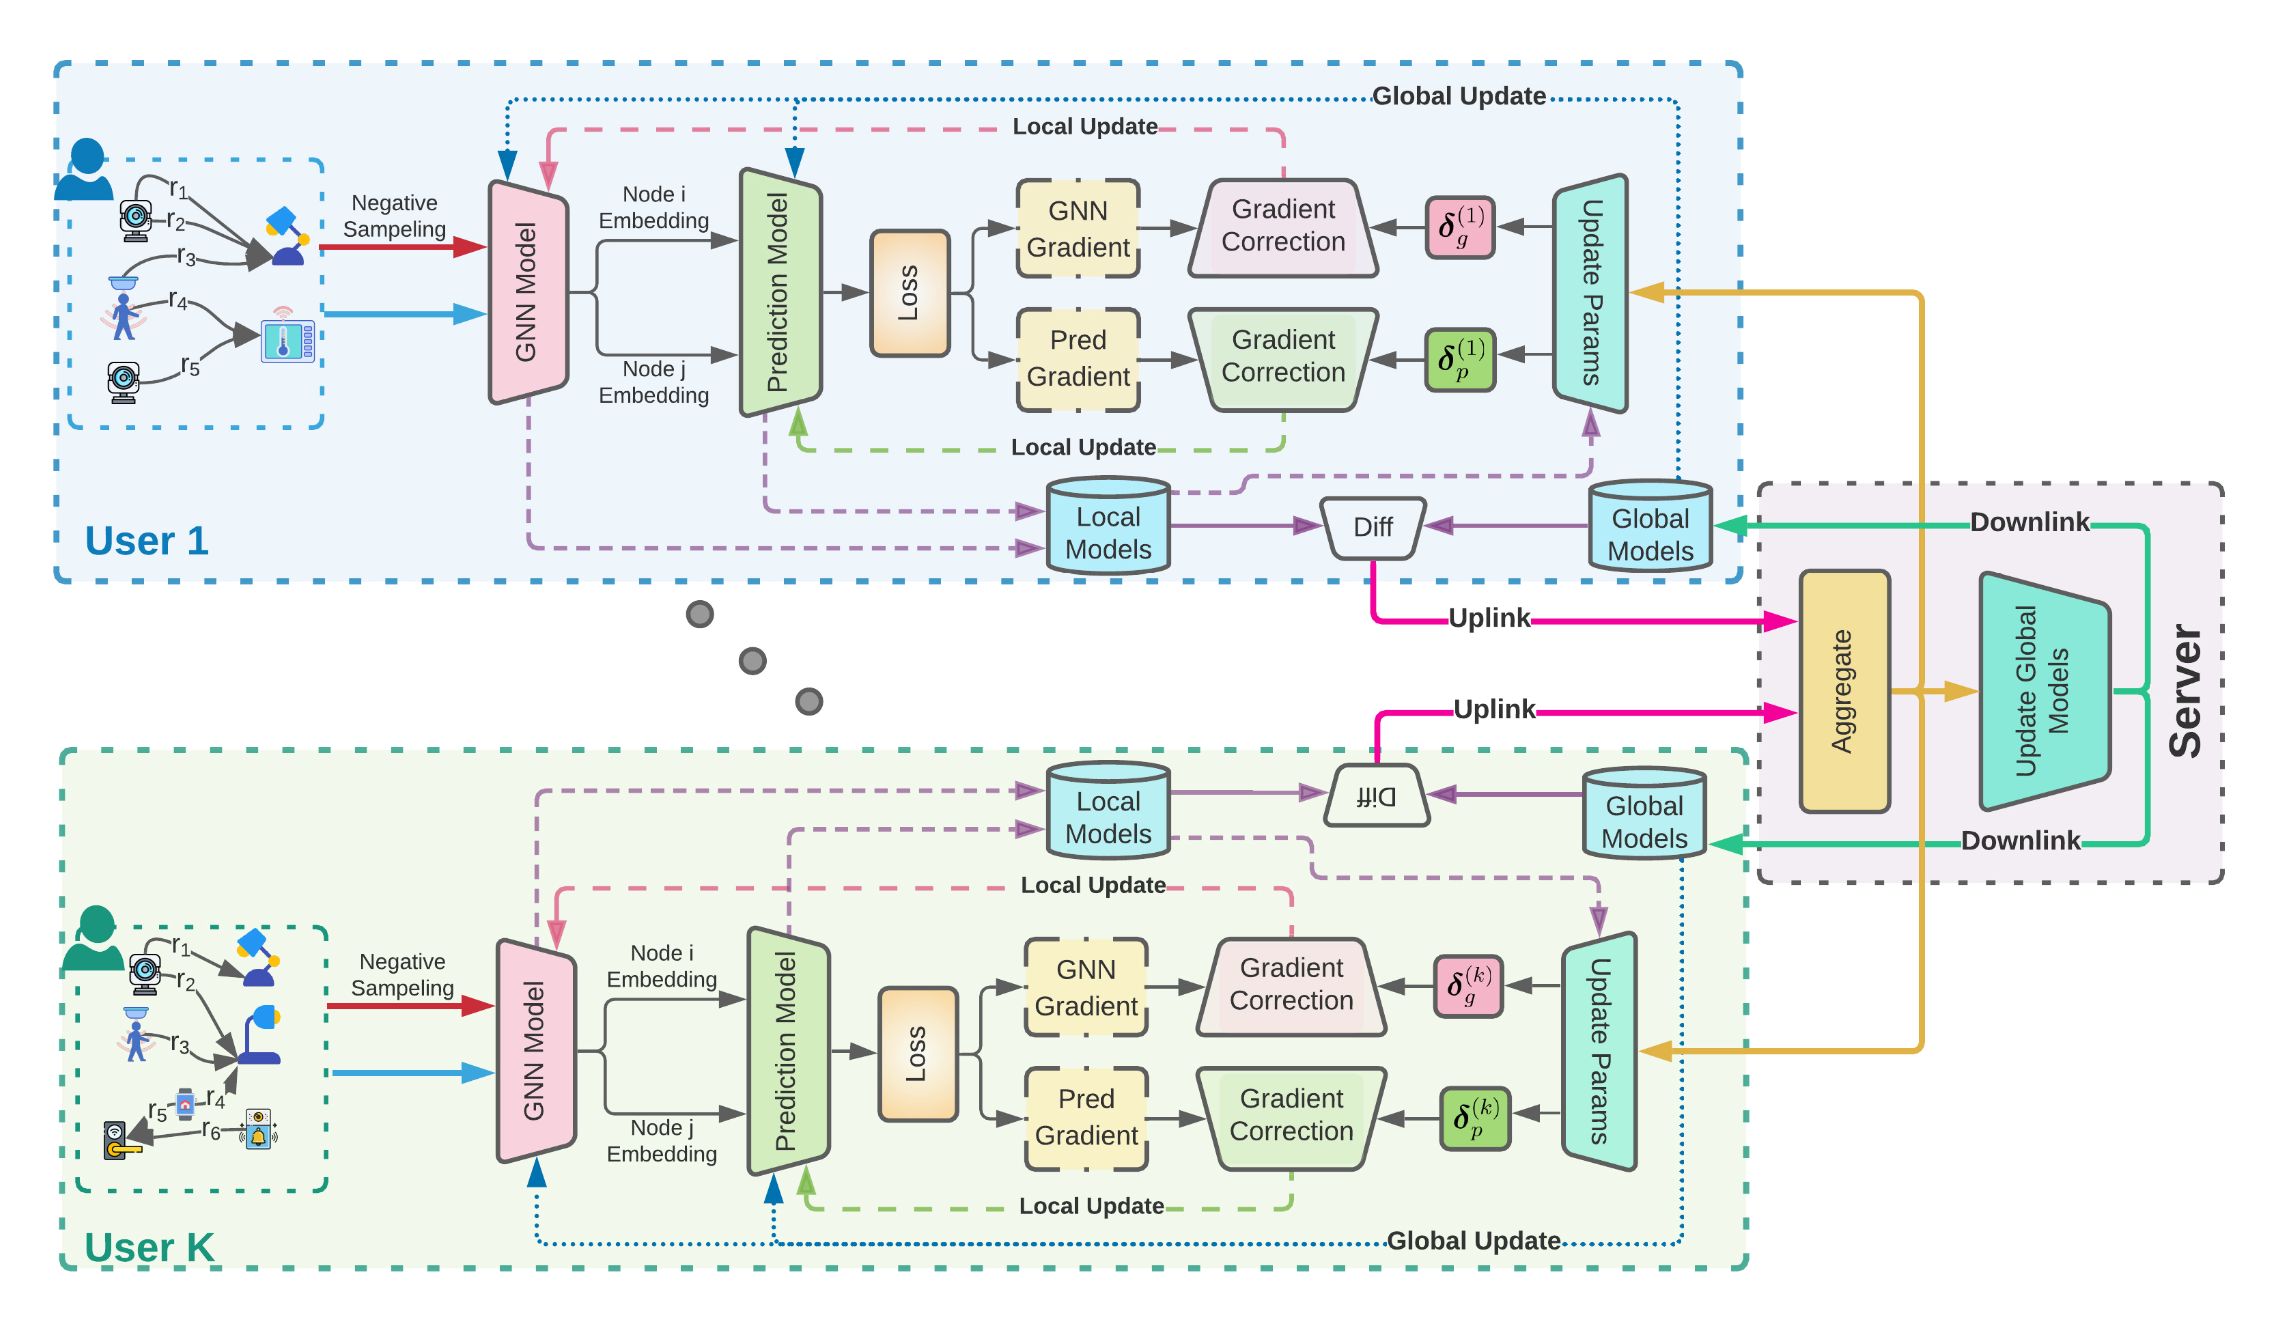
\includegraphics[width=\linewidth]{./assets/images/fedrule-architecture}
  \caption[Η αρχιτεκτονική του FedRule]{Η γενική αρχιτεκτονική του FedRule: κάθε χρήστης έχει το δικό του τοπικό μοντέλο GNN και prediction, τα βάρη των οποίων στέλνονται στον server για aggregation και update, ενώ τα τοπικά τους gradients διορθώνονται από τις παραμέτρους διόρθωσης \cite{yao_fedrule_2022}.}
  \label{fig:fedrule-architecture}
\end{figure}

\subsubsection{Η διαδικασία του training}
Εδώ εντοπίζεται η μεγαλύτερη διαφοροποίηση μεταξύ του paper της Wyze και της υλοποίησής της. Ενώ το paper αναπτύσσει έναν αλγόριθμο Federated Learning, τον FedRule, ως απάντηση στα ζητήματα ιδιωτικότητας και ετερογένειας των δεδομένων, η υλοποίηση που παρείχε στον διαγωνισμό εφαρμόζει τον αλγόριθμο GraphRule, μία αμιγώς centralized μέθοδο εκμάθησης. Δεν υπάρχει κάποια ουσιαστική διαφορά στα μοντέλα μηχανικής μάθησης ή τα datasets, παρά μόνο στην ενορχήστρωση της εκπαίδευσης. Εδώ, ο κεντρικός server έχει πλήρη πρόσβαση σε όλα τα δεδομένα όλων των χρηστών και εκπαιδεύει τα μοντέλα σε κεντρικό επίπεδο. Η στρατηγική aggregation FedRule περιγράφεται στο paper \cite{yao_fedrule_2022} αλλά δεν εμφανίζεται στον κώδικα.

\subsubsection{Μετρικές}\label{sssec:metrics}
Η υλοποίηση της Wyze στηρίζει την αξιολόγησή της σε τρεις μετρικές: το Σφάλμα (Loss), το Area Under the Curve (AUC) και το Mean Rank (MR), ενώ το paper κάνει χρήση και της μετρικής HitRate@N.

Ως συνάρτηση σφάλματος χρησιμοποιείται η Binary Cross Entropy (BCE) Loss \cite{goodfellow_deep_2016}, η πιο συνήθης μετρική σφάλματος για προβλήματα ταξινόμησης με έξοδο κατανομή πιθανοτήτων στο διάστημα $[0,1]$ (όπως στο δικό μας πρόβλημα, στο οποίο το μοντέλο εξάγει τις πιθανότητες μία ορισμένη ακμή να έχει χρησιμότητα για τον χρήστη). Όσο μικρότερη η BCE, τόσο πιο ακριβές το μοντέλο. Ο μαθηματικός της τύπος ορίζεται ως: $$L_{BCE} = -\frac{1}{N} \sum_{i=1}^{N} \left[ y_i \log(p_i) + (1 - y_i) \log(1 - p_i) \right]$$ όπου $N$ το πλήθος των δειγμάτων, $y_i$ η πραγματική ετικέτα (1 για υπαρκτό κανόνα, 0 για μη υπαρκτό) και $p_i$ η προβλεπόμενη πιθανότητα από το μοντέλο.

Η μετρική AUC ποσοτικοποιεί την ικανότητα του μοντέλου να διακρίνει τα πραγματικά θετικά δείγματα (True Positives, TP) από τα ψευδώς θετικά (False Positives, FP, δηλαδή τις τεχνητά παραγόμενες αρνητικές ακμές κατά την διαδικασία του negative sampling). Υπολογίζεται ως το εμβαδόν κάτω από την καμπύλη ROC (Receiver Operating Characteristic) \cite{fawcett_introduction_2006}, η οποία σχεδιάζεται τοποθετώντας στον άξονα Υ το ποσοστό των True Positives (TPR ή Sensitivity) και στον άξονα Χ το ποσοστό των False Positives (FPR, που ισούται με 1 - Specificity). Μια τυχαία ταξινόμηση χαράσσει την ευθεία $y=x$ (AUC = 0.5), ενώ ένα τέλειο μοντέλο αγγίζει εμβαδόν 1.

Το Mean Rank (MR) \cite{bordes_translating_2013} εκφράζει τη μέση θέση στην οποία κατατάσσεται ο πραγματικός/επιθυμητός κανόνας μέσα στη φθίνουσα λίστα των πιθανοτήτων που παρήγαγε το δίκτυο. Μικρότερες τιμές υποδηλώνουν καλύτερη απόδοση. Αξίζει να σημειωθεί πως στην υλοποίηση της Wyze η αρίθμηση ξεκινά από το 0 (τέλεια πρόβλεψη: MR=0), σε αντίθεση με την καθιερωμένη ακαδημαϊκή πρακτική όπου η κορυφαία θέση ορίζεται ως 1η (MR=1).

Τέλος, το HitRate@N \cite{bordes_translating_2013} μετρά το ποσοστό των περιπτώσεων όπου ο σωστός κανόνας εμφανίζεται μέσα στις κορυφαίες $N$ προτάσεις του συστήματος. Παρότι η αρχική υλοποίηση κώδικα δεν το υπολογίζει αυτόματα, η μετρική αυτή είναι θεμελιώδης τόσο στην ευρύτερη βιβλιογραφία όσο και στην παρούσα εργασία, καθώς αντικατοπτρίζει άμεσα την πρακτική χρησιμότητα του συστήματος για τον τελικό χρήστη.

\subsection{Οι αδυναμίες του μοντέλου}\label{ssec:weaknesses}
Η υλοποίηση της Wyze θέτει μία ακέραια βάση για πειραματισμό, ωστόσο καθαυτή παρουσιάζει μία κρίσιμη αδυναμία: την μη ενσωμάτωση των τύπων των προϋπαρχόντων κανόνων κατά την εκπαίδευση του GNN. Παρότι το embedding των γράφων αφομοιώνει επιτυχώς τα χαρακτηριστικά των κόμβων (αναγνωρίζοντας, για παράδειγμα, ότι μια κάμερα σχετίζεται συχνά με αισθητήρες), το μοντέλο αντιμετωπίζει τις ακμές του γράφου ως απλές δυαδικές συνδέσεις, δεν κωδικοποιεί δηλαδή τον τύπο της προϋπάρχουσας αλληλεπίδρασης. Σε ένα σύνολο πραγματικών δεδομένων που αγγίζει το 1.000.000 κανόνων, η αδυναμία αξιοποίησης αυτής της πλούσιας συντακτικής πληροφορίας στερεί από το δίκτυο σημαντικό context, αναγκάζοντάς το να εξάγει συμπεράσματα αποκλειστικά από την τοπολογία, γεγονός που περιορίζει δραστικά τη μέγιστη δυνατή επίδοσή του.

\section{Η δεύτερη θέση του διαγωνισμού}\label{sec:second-place}
Σε αυτή την Ενότητα αναλύεται η προσέγγιση του διαγωνιζόμενου που κατέκτησε τη δεύτερη θέση στον διαγωνισμό \cite{conti_conti748wyze-rule-recommendation_2024}. Σημειώνεται πως η λύση της πρώτης θέσης δεν κατέστη δυνατό να εντοπιστεί δημόσια, και γι' αυτό επιλέχθηκε η αμέσως χαμηλότερη σε κατάταξη. Πρόκειται για μία centralized υλοποίηση που εφαρμόζει σημαντικές αρχιτεκτονικές βελτιώσεις σε όλο το pipeline της εκπαίδευσης. Καθώς πρόκειται για διαγωνισμό επιδόσεων, ο διαγωνιζόμενος έστρεψε την προσοχή του στην βελτιστοποίηση του σκορ του και όχι στα ζητήματα ιδιωτικότητας των χρηστών, ωστόσο η υλοποίησή του εξακολουθεί να παρουσιάζει έντονο ακαδημαϊκό ενδιαφέρον.

Η υλοποίηση αξιοποιεί την βιβλιοθήκη PyTorch Geometric (PyG) \cite{fey_fast_2019, pyg_software} για την διαχείριση των γράφων και ακολουθεί επί το πλείστον τα ίδια βήματα με την baseline υλοποίηση της Wyze, με μερικές διαφοροποιήσεις που θα παρουσιαστούν παρακάτω.

Η ειδοποιός διαφορά που οδήγησε την υλοποίηση αυτή στην δεύτερη θέση είναι η αφομοίωση των τύπων των ακμών κάθε γράφου, που ήταν η μεγαλύτερη παράλειψη του μοντέλου της Wyze, όπως αναλύθηκε στην \autoref{ssec:weaknesses}. Συγκεκριμένα, το δίκτυο αυτό δεν χρησιμοποιεί embeddings μόνο για τους κόμβους, αλλά ενσωματώνει πληροφορία και στις ακμές (edge embeddings) \cite{schlichtkrull_modeling_2018}, καθοδηγώντας το μοντέλο να αξιοποιήσει τα λανθάνοντα μοτίβα στους προϋπάρχοντες κανόνες μεταξύ των συσκευών των χρηστών. Αυτή η πυκνή πληροφορία στην συνέχεια αθροίζεται μέσω μιας custom aggregation συνάρτησης σε κάθε κόμβο. Ως αποτέλεσμα, το μοντέλο μαθαίνει το πλήρες πλαίσιο αλληλεπίδρασης κάθε συσκευής. Για παράδειγμα, δεν μαθαίνει απλώς ότι μία κάμερα συνδέεται με ένα σύστημα συναγερμού, αλλά κατανοεί ειδικά ότι η «αναγνώριση κίνησης» είναι αυτή που πυροδοτεί την ενεργοποίησή του.

Παράλληλα, στοχευμένες τροποποιήσεις στο υπόλοιπο pipeline οδηγούν σε περαιτέρω βελτιστοποιήσεις. Η υλοποίηση αξιοποιεί την βιβλιοθήκη Pandas \cite{mckinney_data_2010, pandas_software} για την ταχύτερη φόρτωση και ομαδοποίηση των συσκευών και κανόνων ανά χρήστη. Αφού οι γράφοι έχουν δημιουργηθεί, ο αλγόριθμος επιλέγει τυχαία και αποκρύπτει ακριβώς μία ακμή από τον γράφο κάθε χρήστη (leave-one-out strategy), με σκοπό το μοντέλο να την προβλέψει κατά την εκπαίδευσή του, μια διαδικασία που περιγράφεται στο paper της Wyze αλλά δεν υλοποιείται. Αντίστοιχα, το negative sampling περιορίζεται σε μία μόνο τεχνητή (ψευδή) ακμή ανά γράφο για να εξισορροπήσει την μία πραγματική που αφαιρέθηκε.

Επιπλέον, για την επιτάχυνση και σταθεροποίηση της σύγκλισης, ενσωματώνεται ένας δυναμικός ρυθμός μάθησης (dynamic learning rate) \cite{ruder_overview_2016}, ο οποίος αναπροσαρμόζεται βάσει του validation loss. Η συνάρτηση σφάλματος BCE είναι επίσης προσαρμοσμένη αναλυτικά (με απευθείας χρήση λογαρίθμων) ώστε να λαμβάνει υπόψη όλες τις πιθανές κατηγορίες των ακμών, αξιοποιώντας τα προαναφερθέντα edge embeddings. Κατά την φάση της αξιολόγησης, το σύστημα παράγει όλους τους πιθανούς συνδυασμούς κανόνων μεταξύ των διαθέσιμων συσκευών (πλήρεις γράφοι) \cite{bordes_translating_2013} και υπολογίζει την πιθανότητά τους, κάτι που καθιστά τον εντοπισμό της κρυμμένης ακμής πολύ πιο δύσκολο, αλλά ταυτόχρονα απόλυτα ρεαλιστικό.

Τέλος, η κύρια μετρική αξιολόγησης δεν είναι το Mean Rank, αλλά το αντίστροφό του (Mean Reciprocal Rank, MRR) \cite{craswell_mean_2009}, το οποίο έχει την μαθηματική ιδιότητα να εφαρμόζει αυστηρότερη ποινή σε μοντέλα που κατατάσσουν τον πραγματικό κανόνα χαμηλά στη λίστα των προτάσεων, αναγκάζοντας το δίκτυο να δώσει προτεραιότητα στην εύρεσή του. Οι παραπάνω βελτιστοποιήσεις συμβάλλουν στην αύξηση της ταχύτητας ή της απόδοσης του μοντέλου, όμως δημιουργούν και μια πιο στιβαρή βάση για την αξιολόγησή του.

Η θεμελιώδης αδυναμία της υλοποίησης αυτής έγκειται ωστόσο στην centralized φύση της. Όπως έχει αναδειχθεί και στις προηγούμενες Ενότητες, ένας από τους σημαντικότερους στόχους του διαγωνισμού αλλά και των πραγματικών IoT συστημάτων είναι η διασφάλιση της προστασίας των προσωπικών δεδομένων των χρηστών. Για να επιτευχθεί αυτός ο σκοπός, είναι απαραίτητη η χρήση ενός federated περιβάλλοντος. Η παρούσα διπλωματική εργασία γεφυρώνει αυτό ακριβώς το χάσμα: απομονώνει τις εξαιρετικές αρχιτεκτονικές βελτιστοποιήσεις της δεύτερης θέσης, ενορχηστρώνοντάς τες όμως σε ένα federated πλαίσιο.